\documentclass[conference]{IEEEtran}

\usepackage{amsmath}
\usepackage{graphicx}
%\usepackage[backend=bibtex,style=chem-rsc]{biblatex}
\usepackage{lettrine}
\usepackage{cite}
\usepackage{float}
\usepackage{blindtext}
\usepackage{eso-pic}
\usepackage[utf8]{inputenc}
\usepackage[english]{babel}
\usepackage[numbers]{natbib}
\usepackage{hyperref}
\usepackage{booktabs}
\usepackage{textcomp}
\usepackage{filecontents}
\newcommand\tab[1][1cm]{\hspace*{#1}}
\newcommand\AtPageUpperMyright[1]{\AtPageUpperLeft{%
    \put(\LenToUnit{0.5\paperwidth},\LenToUnit{-1cm}){%
     \parbox{0.5\textwidth}{\raggedleft\fontsize{9}{11}\selectfont #1}}%
    }}%
    \newcommand{\conf}[1]{%
    \AddToShipoutPictureBG*{%
    \AtPageUpperMyright{#1}}
}

\title{cdma_rx}

\author{
  \IEEEauthorblockN{Armaan Kohli}
  \IEEEauthorblockA{\textit{Department of Electrical Engineering} \\
\textit{The Cooper Union for the Advancement of Science and Art}\\
New York City, United States \\
kohli@cooper.edu\\
\href{github.com/armaank/wi-comms}{https://github.com/armaank/wi-comms}}}

\begin{document}
\title{CDMA Receiver for Secret Messages}

\maketitle
\conf{ECE-408: WIRELESS COMMUNICATIONS, MARCH 2020}

\begin{abstract}
 We design a receiver for a simple Code Division Multiple Access (CDMA) wireless system. We successfully decode and interpret a secret message transmitted over the simple CDMA system, and recover both phase and frequency offsets. 
\end{abstract}

\begin{IEEEkeywords}
CDMA, maximum length sequences, Wash encoding, secret messages
\end{IEEEkeywords}

\section{Introduction}
\lettrine[findent=2pt]{\textbf{C}}{ }ode Division Multiple Access (CDMA) is a multiple-access technique that leverages spreading codes to allow multiple users to receive data across the same channel. In order to design a receiver for a CDMA system, one must consider pilot synchronization, frequency and phase offsets, and the framing structure of the packets. In our system, a secret message is encoded into bits modulated via binary phase shift keying (BPSK) and encoded via an 8-ary Walsh code. A pilot, consisting of all zeros, is on the 0th Walsh channel, and the data is on the 5th Walsh channel. The data is then spread using an maxium length sequence, henceforth known as an M-sequence. The resultant bit-stream is then oversampled, filtered and transmitted. At the receiver, we must design a system to take the received frames and decode the hidden message.

\section{CDMA Decoder}
After filtering the received signal with a raised-root cosine filter and decimation by four according to the oversampling factor, the first challenge in building an effective CDMA decoder was to synchronize the received signal. This was done by computing the cross correlation with an M-sequence was generated from the same polynomial. Using the autocorrelation, we could see precisely where the pilot sequence began. 

Then, using the pilots, we performed phase and frequency correction. Since the first and last frames sent consist of pilot signals, we computed the relative frequency and phase offset between the first and last pilots as an estimate. Using these estimates, we corrected the received constellation. The effect of the phase and frequency correction is illustrated in Fig. \ref{fig:const}
\begin{figure}[htbp]
\centerline{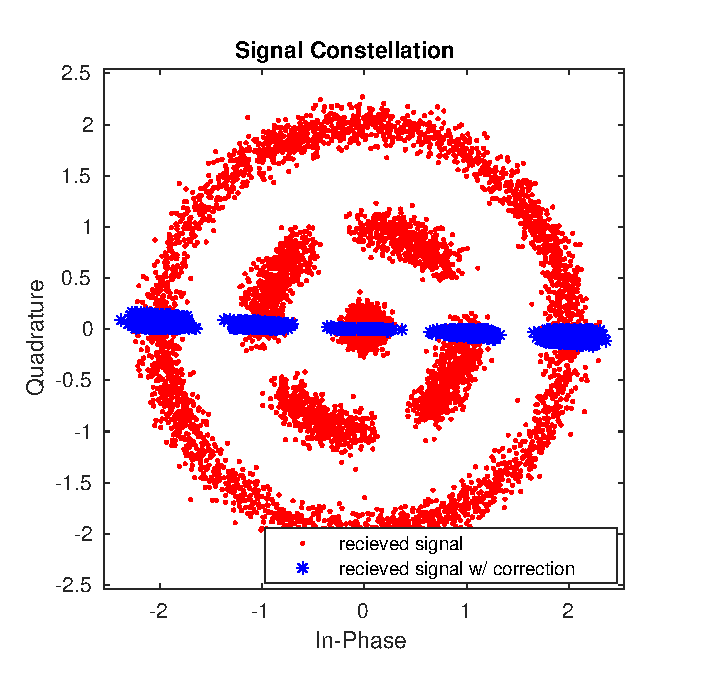
\includegraphics[scale=.75]{./media/constellation.eps}}
\caption{Constellation diagrams of the received signal, pre and post phase and frequency correction }
\label{fig:const}
\end{figure}
Finally, we despread and decoded the data frames. This consisted of demodulation and de-scrambling. We used a custom BPSK demodulator to map the received symbols into Walsh-encoded values. The de-scrambling was done by XORing the demodulated data with the same M-sequence. We then decode the data frames by multiplying by the 5th Walsh channel, convert the binary sequence into characters and interpret the secret message.


\section{Results} 
We determined that the frequency offset was 999.38 Hz, the phase offset was -43.9\textdegree. We received the following secret message: \texttt{Happiness can be found, even in the darkest of times, if one only remembers to turn on the light.} This refers to my inability to operate switches, both for lights and projector screens, first demonstrated on the first day of class. It is also a reference to \textit{Harry Potter and the Prisoner of Azkaban}, a quote by Albus Dumbledore, the Headmaster of the Hogwarts School of Witchcraft and Wizardry. What a double entendre!

\section{Conclusion} 
We designed a CDMA receiver and successfully recovered the transmitted secret message.  
%\bibliographystyle{unsrt}
%\bibliography{bib}
\end{document}